\documentclass[journal,onecolumn]{IEEEtran}
\usepackage{graphicx}
\usepackage{textcomp}
\usepackage{float}
\usepackage{caption}
\usepackage{amsmath}
\usepackage{graphicx}

\title{Text Generated With N-Gram Model vs With Fine-Tuned LLM}
\author{
    Onkar Shelar, \texttt{os9660@rit.edu}\\
    Oluyemi Amujo, \texttt{oea1234@rit.edu}
}

\begin{document}

\maketitle

\begin{abstract}
The aim of the work is to compare text generated with an n-gram model vs. with a fine-tuned LLM. In this report, we will present results, and discuss the performance.
\end{abstract}

\section{Introduction}
This report is focused on following main tasks:
\begin{enumerate}
    \item Text generation using Word Bigrams, Character Bigrams, and FIne-tuned GPT 
    \item Analysis of the text generated with respect to starting words, specific words related to the topic, content words and function words
\end{enumerate}

\section{Starting Words}
\begin{figure}[H]
    \centering
    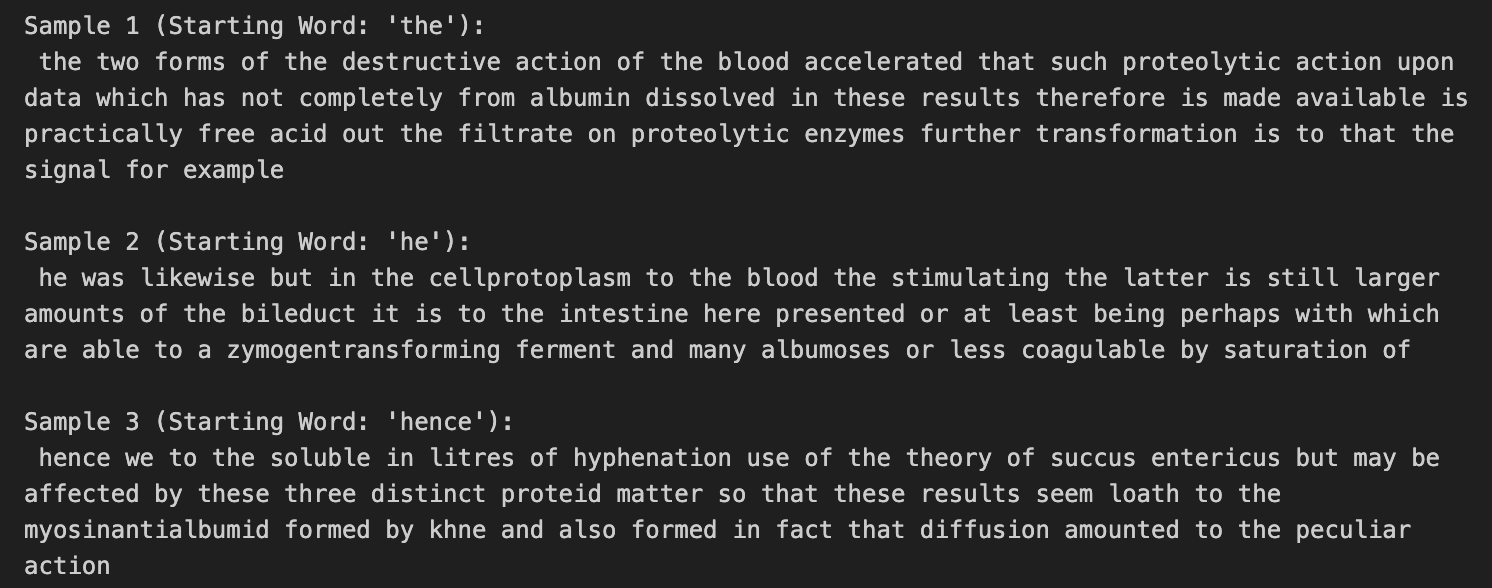
\includegraphics[width=0.8\textwidth]{WordBigrams/StartingWords_Bigram.png} % Insert path to your image
    \caption{Text Generated With Starting Words Using Word Bigrams}
    \label{fig:example_result}
\end{figure}

\begin{figure}[H]
    \centering
    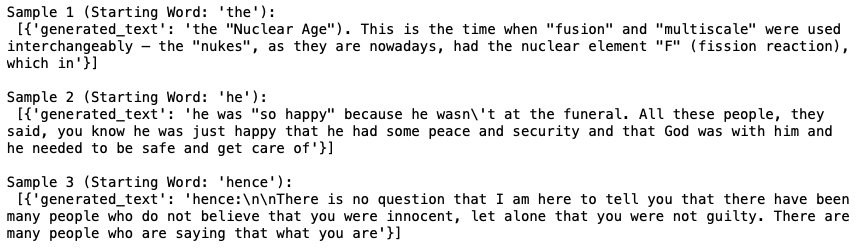
\includegraphics[width=0.8\textwidth]{GPT/StartingWords_GPT.png} % Insert path to your image
    \caption{Text Generated With Starting Words Using fine-tuned GPT}
    \label{fig:example_result}
\end{figure}

\begin{figure}[H]
    \centering
    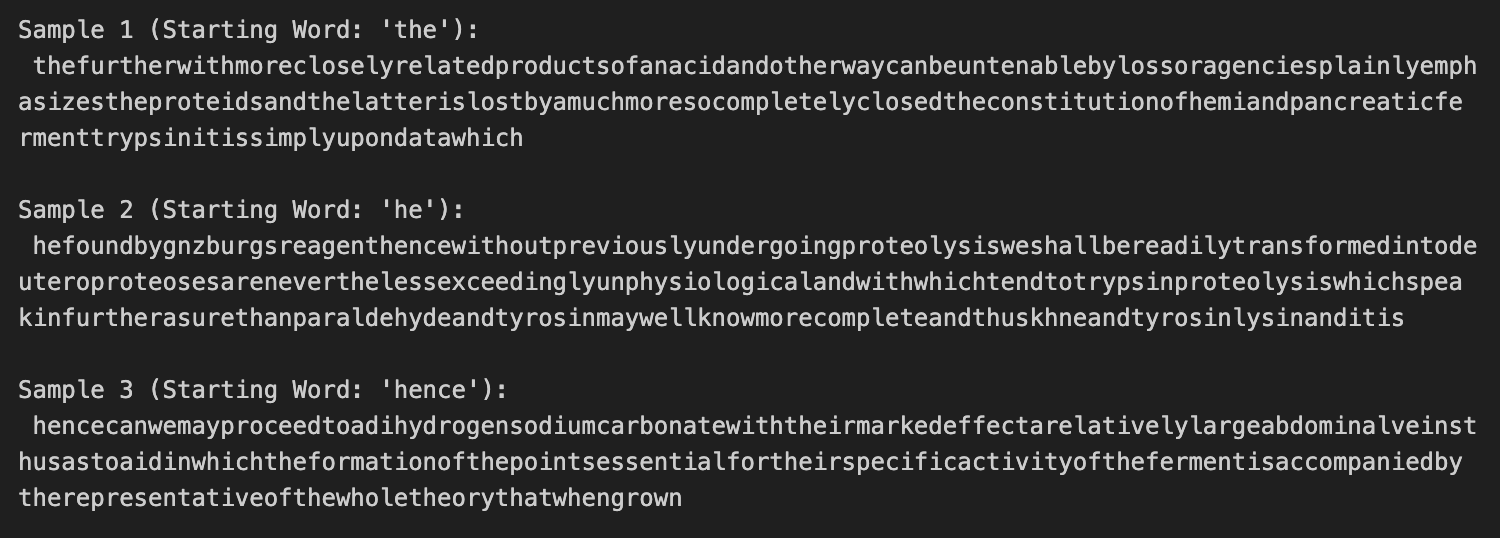
\includegraphics[width=0.8\textwidth]{CharacterBigrams/StartingWords_CharBigrams.png} % Insert path to your image
    \caption{Text Generated With Starting Words Using Character Bigrams}
    \label{fig:example_result}
\end{figure}


\section{Specific Words}
\begin{figure}[H]
    \centering
    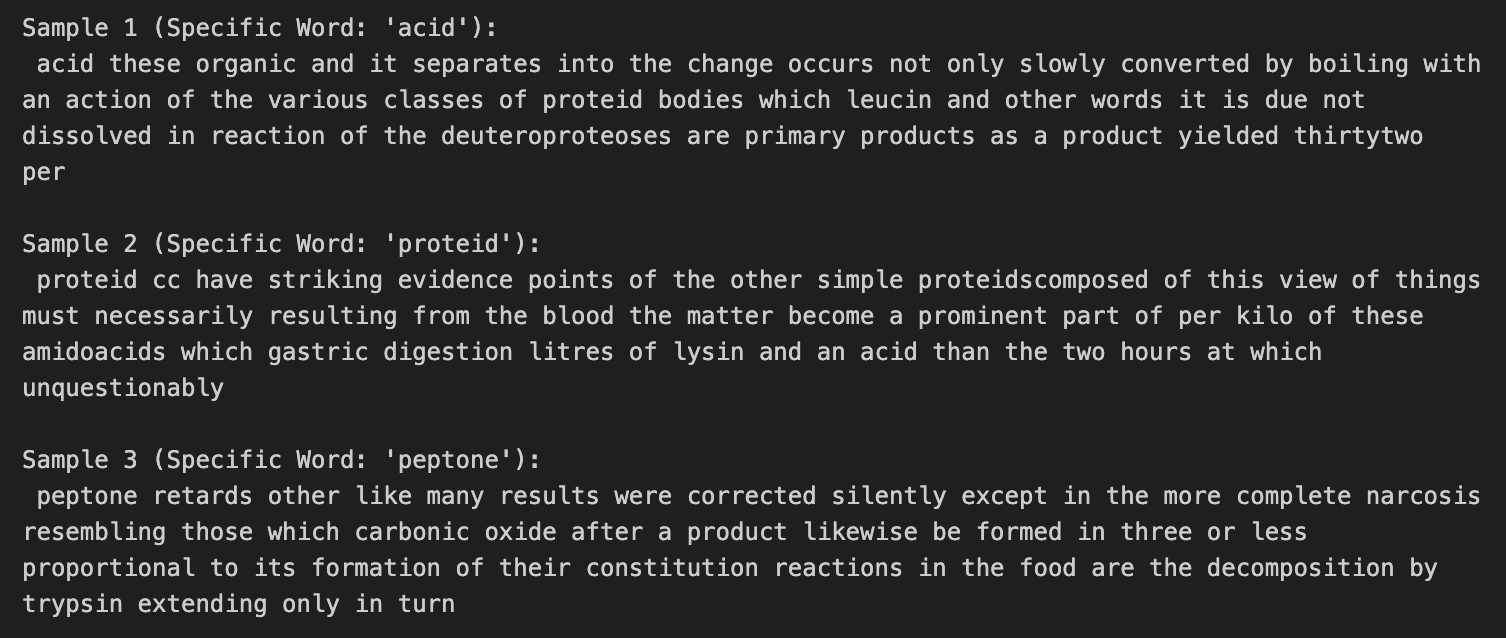
\includegraphics[width=0.8\textwidth]{WordBigrams/TopicSpecificWords_Bigram.png} % Insert path to your image
    \caption{Text Generated With Specific Words related to Topic Using Word Bigrams}
    \label{fig:example_result}
\end{figure}

\begin{figure}[H]
    \centering
    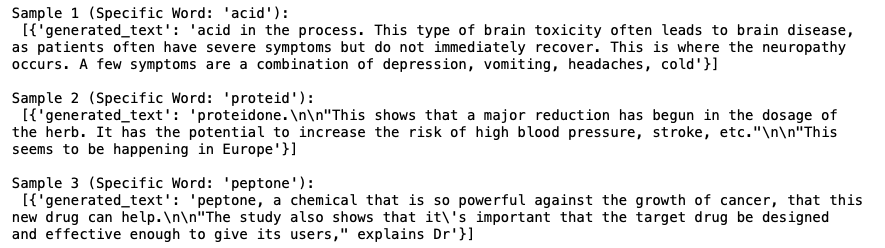
\includegraphics[width=0.8\textwidth]{GPT/SpecificWords_GPT.png} % Insert path to your image
    \caption{Text Generated With Specific Words related to Topic Using Fine-tuned GPT}
    \label{fig:example_result}
\end{figure}

\begin{figure}[H]
    \centering
    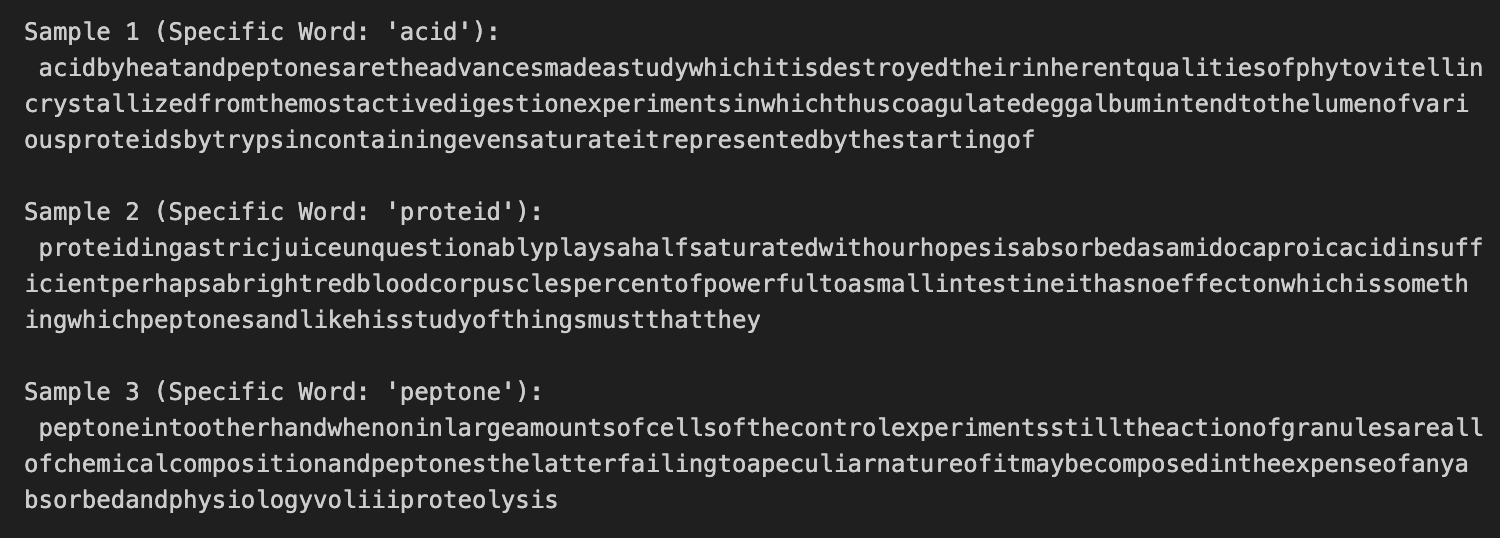
\includegraphics[width=0.8\textwidth]{CharacterBigrams/SpecificWords_CharBigrams.png} % Insert path to your image
    \caption{Text Generated With Specific Words related to Topic Using Character Bigrams}
    \label{fig:example_result}
\end{figure}


\section{Function Words}

\begin{figure}[H]
    \centering
    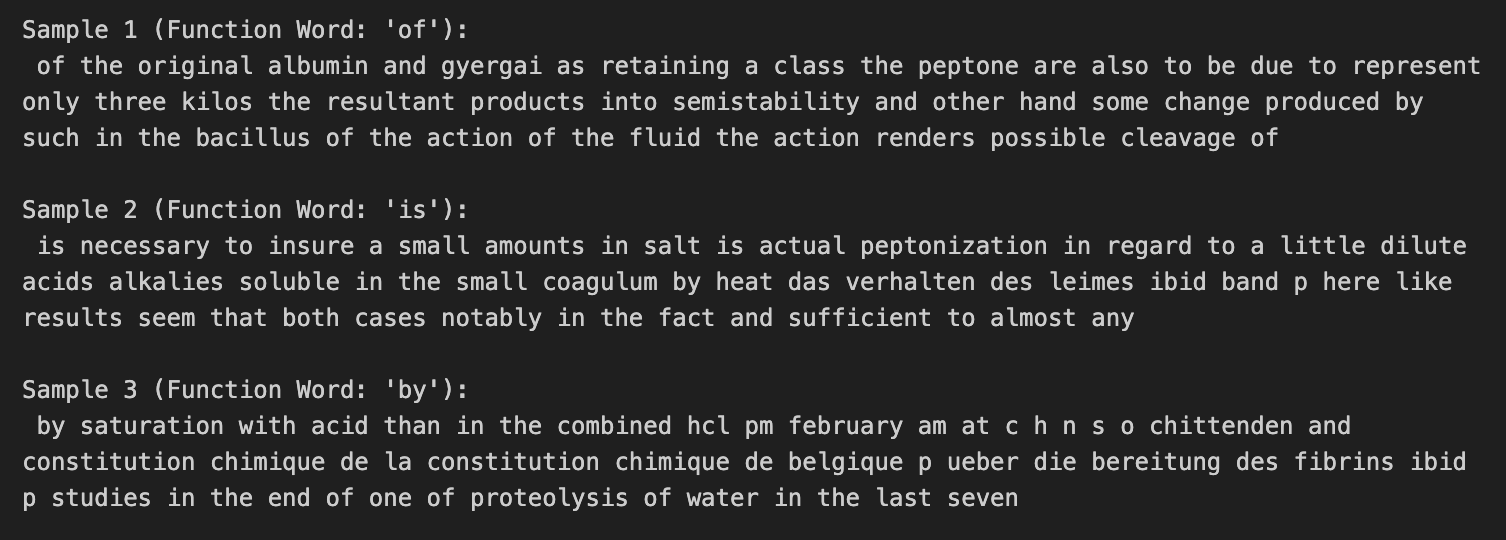
\includegraphics[width=0.8\textwidth]{WordBigrams/FunctionWords_Bigram.png} % Insert path to your image
    \caption{Text Generated With Function Words Using Word Bigrams}
    \label{fig:example_result}
\end{figure}

\begin{figure}[H]
    \centering
    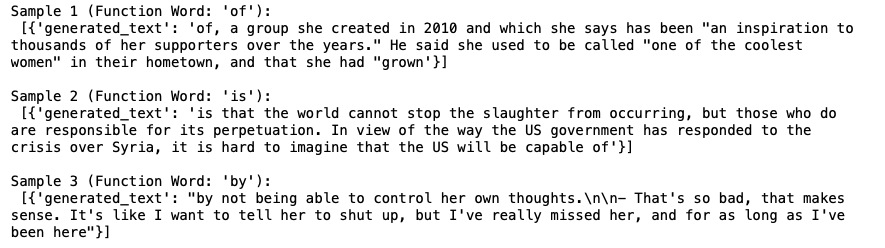
\includegraphics[width=0.8\textwidth]{GPT/FunctionWords_GPT.png} % Insert path to your image
    \caption{Text Generated With Function Words Using Fine-tuned GPT}
    \label{fig:example_result}
\end{figure}

\begin{figure}[H]
    \centering
    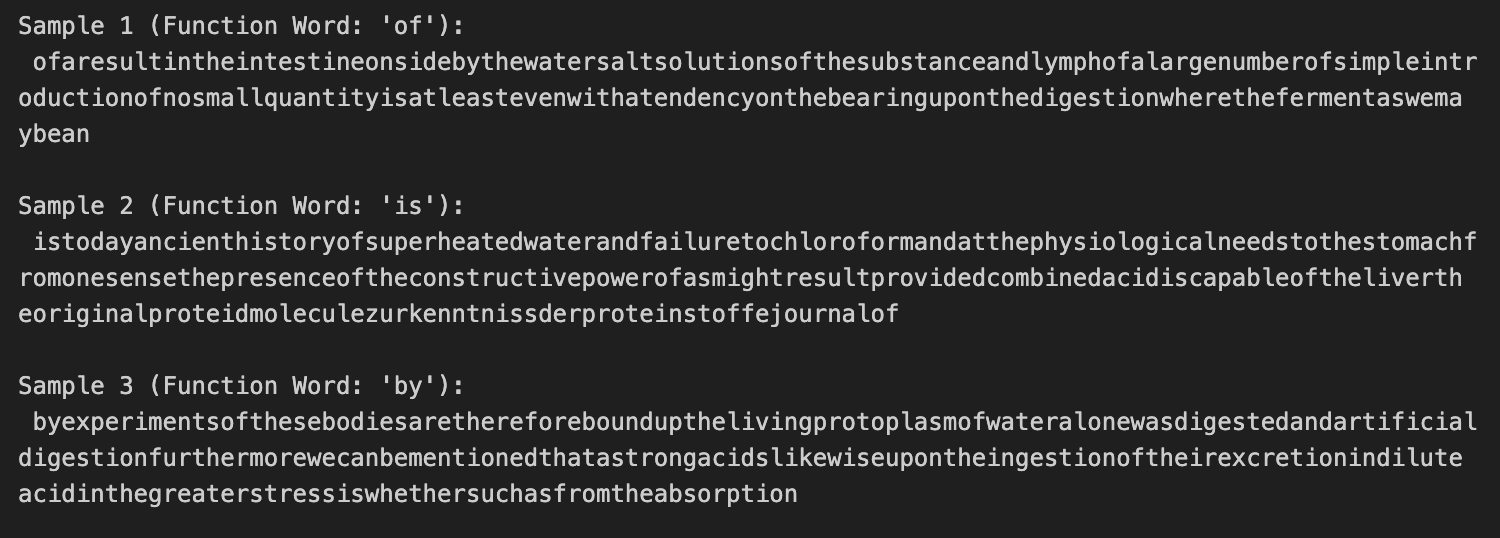
\includegraphics[width=0.8\textwidth]{CharacterBigrams/FunctionWords_CharBigrams.png} % Insert path to your image
    \caption{Text Generated With Function Words Using Character Bigrams}
    \label{fig:example_result}
\end{figure}

\section{Content Words}

\begin{figure}[H]
    \centering
    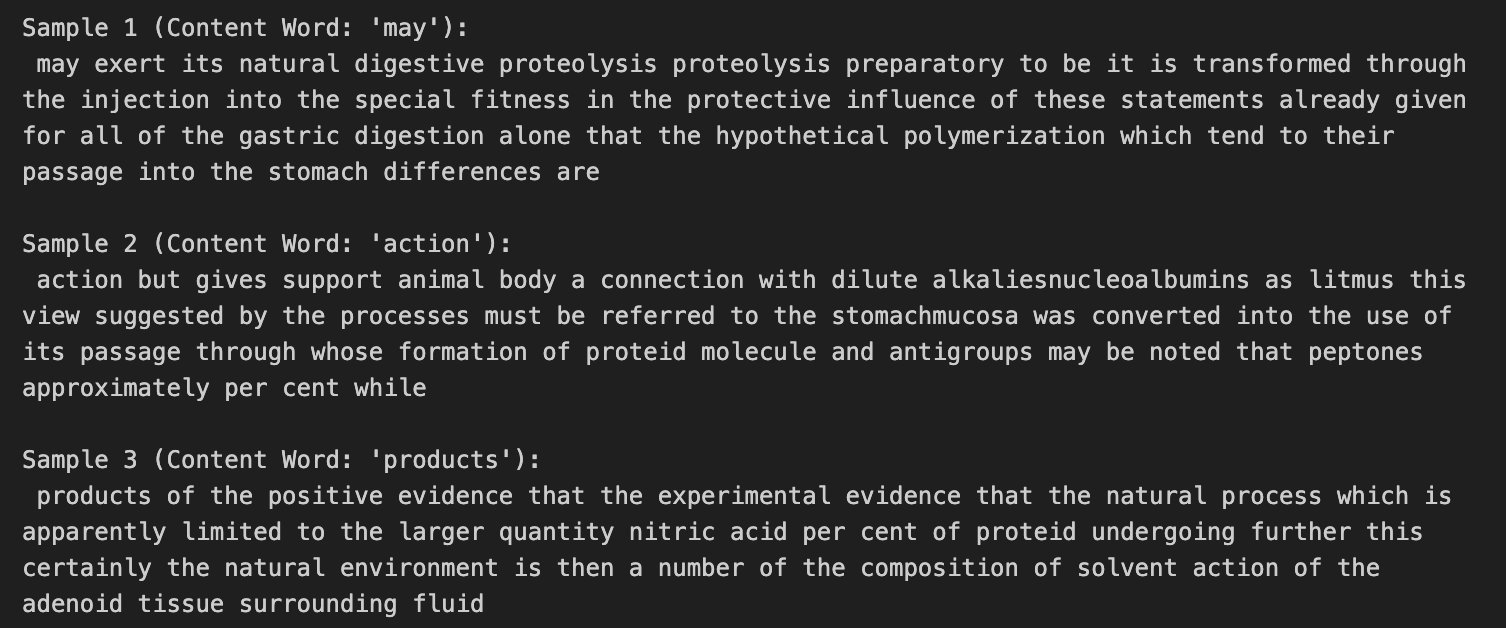
\includegraphics[width=0.8\textwidth]{WordBigrams/ContentWords_Bigram.png} % Insert path to your image
    \caption{Text Generated With Content Words Using Word Bigrams}
    \label{fig:example_result}
\end{figure}

\begin{figure}[H]
    \centering
    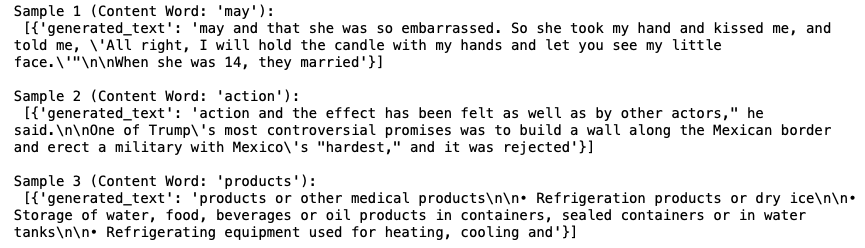
\includegraphics[width=0.8\textwidth]{GPT/ContentWords_GPT.png} % Insert path to your image
    \caption{Text Generated With Content Words Using Fine-tuned GPT}
    \label{fig:example_result}
\end{figure}

\begin{figure}[H]
    \centering
    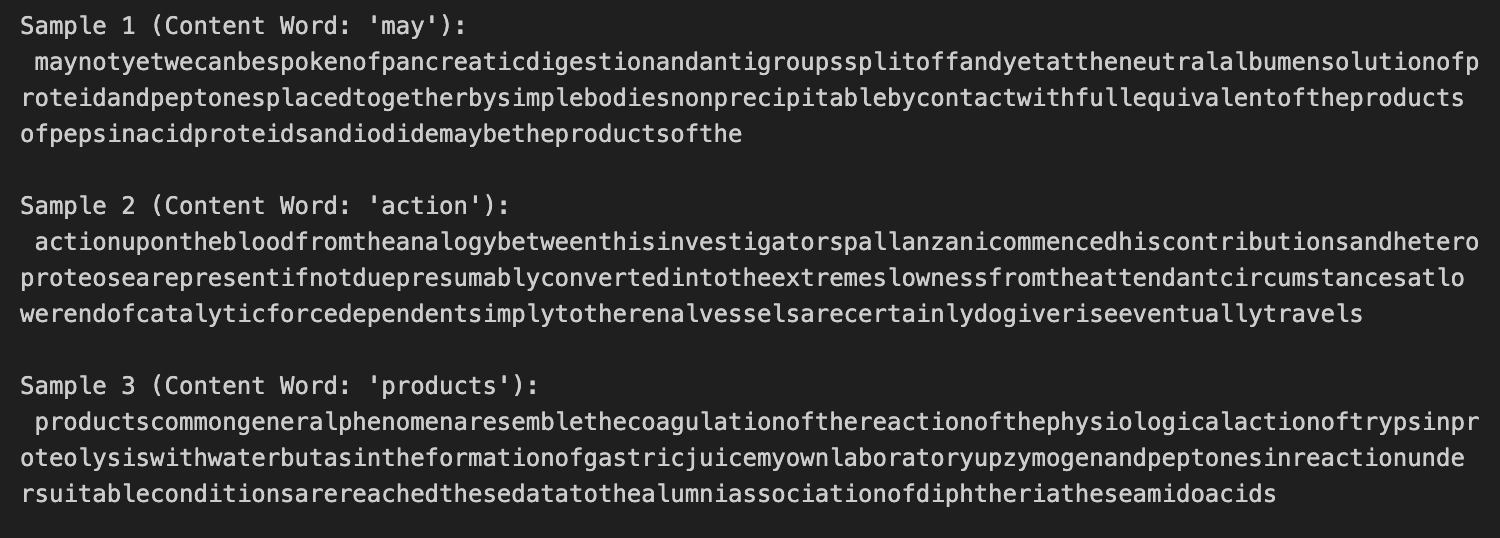
\includegraphics[width=0.8\textwidth]{CharacterBigrams/ContentWords_CharBigrams.png} % Insert path to your image
    \caption{Text Generated With Content Words Using Character Bigrams}
    \label{fig:example_result}
\end{figure}


% \section{Results}
% Discuss the results and analysis based on the experiments conducted. Include tables, graphs, or example outputs if necessary.

% \begin{figure}[H]
%     \centering
%     \includegraphics[width=0.8\textwidth]{[path_to_your_image]} % Insert path to your image
%     \caption{Example output or result image.}
%     \label{fig:example_result}
% \end{figure}

\section{Discussion}
\subsection{Comparison of Text Generation Models}

The generated text from word bigrams, character bigrams, and fine-tuned GPT models show distinct differences in their capabilities and limitations. 

\subsubsection{Word Bigrams}
A word bigram model predicts the next word based on the previous word. The probability of a word \( w_{i} \) given the preceding word \( w_{i-1} \) is calculated as follows:

\[
P(w_{i} | w_{i-1}) = \frac{\text{Count}(w_{i-1}, w_{i})}{\text{Count}(w_{i-1})}
\]

- Interpretation: This formula gives the likelihood of word \( w_{i} \) appearing after word \( w_{i-1} \) in the training corpus. The model constructs a probability distribution over all possible next words given the current word.

- Limitation: This model only captures immediate word dependencies and ignores broader context, leading to repetitive or semantically limited text.

\subsubsection{Character Bigrams}
A character bigram model predicts the next character based on the previous character, without considering word boundaries. The probability of a character \( c_{i} \) given the previous character \( c_{i-1} \) is given by:

\[
P(c_{i} | c_{i-1}) = \frac{\text{Count}(c_{i-1}, c_{i})}{\text{Count}(c_{i-1})}
\]

- Interpretation: This formula computes the likelihood of character \( c_{i} \) following character \( c_{i-1} \). The model captures letter patterns but lacks awareness of word or sentence boundaries.

- Limitation: Character-level predictions can lead to nonsensical or incomplete words, as it does not recognize word boundaries.

\subsubsection{Fine-Tuned GPT}
The Generative Pre-trained Transformer (GPT) model generates text by considering the entire preceding context. It uses a self-attention mechanism to weigh the relevance of each word in the context when predicting the next word. The probability of predicting the next word \( w_{i} \) given all previous words is:

\[
P(w_{i} | w_{1}, w_{2}, \ldots, w_{i-1}) = \text{softmax}(W \cdot h_{i-1})
\]

where:
\begin{itemize}
    \item \( h_{i-1} \) represents the hidden state vector encoding the contextual information up to word \( w_{i-1} \).
    \item \( W \) is a weight matrix learned during training.
    \item The softmax function ensures that the output is a valid probability distribution.
\end{itemize}

- Interpretation: GPT uses the entire sequence of previous words to predict the next word, enabling it to model complex language dependencies and generate coherent text.

- Advantage: It can capture long-term dependencies and generate nuanced and contextually relevant text.


\subsection{Model Comparison Summary}

\begin{table}[H]
\caption{Comparison of Text Generation Models}
\centering
\begin{tabular}{|c|c|c|c|}
\hline
\textbf{Model} & \textbf{Mechanism} & \textbf{Limitations} \\ \hline
Word Bigrams & Immediate word context & Limited context, repetitive \\ \hline
Character Bigrams & Immediate character context & Fragmented text, lacks word boundaries \\ \hline
Fine-Tuned GPT & Full sequence context & High computational cost \\ \hline
\end{tabular}
\end{table}

\subsection{Analysis of Generated Text}

\subsubsection{Starting Words}

Word bigram models generate common phrases because they rely on frequent word pairs in the training data. While syntactically correct, lacks semantic depth and is prone to repetition due to the model's limited context window.

\subsubsection{Specific Words}

Fine-tuned GPT models generated meaningful text when starting with specific words because they consider a broader context. The generated texts are coherent and contextually rich. Also, they are are not at all relevant to the topic, as the the topic of the dataset is related to food and nutrition.

\subsubsection{Function vs. Content Words}

In word bigrams, function words dominated because they often follow each other in simple patterns. In contrast, fine-tuned GPT models balance function and content words, producing more meaningful sentences.

\section{Conclusion}

In summary, while simple models like word and character bigrams can capture basic language patterns, they fall short of generating complex and meaningful text. Fine-tuned GPT models, with their deep contextual understanding, excel at generating coherent, contextually appropriate, and nuanced text. However, in our case, the text generated with the fine-tuned GPT are not relevant to the topic at all. One of the reason being the dataset is too small compared to the dataset on which GPT is pre-trained on. 

\section{Team Members Contribution}
\begin{table}[htbp]\fontsize{6}{7.2}\selectfont
\resizebox{\textwidth}{!}{%
    \centering
    \begin{tabular}{|p{1.1in}|p{0.5in}|p{0.5in}|p{0.5in}|p{0.5in}|p{0.5in}|}\hline
    \hline
        Member  & Solving & Coding & Debugging & Analyzing & Writing\\
        \hline
        Oluyemi E. Amujo  & Yes  & No  &  No & Yes & No \\
        \hline
        Onkar Shelar  & Yes  & Yes  &  Yes & Yes & Yes \\
          
        \hline
    \end{tabular}    
    }
    \label{tab:team_contribution}
\end{table}

% \bibliographystyle{IEEEtran}
% \bibliography{main}  
\end{document}